\documentclass{article}
\usepackage{amsmath}
\usepackage{tikz}
\usetikzlibrary{arrows.meta}

\begin{document}

\begin{figure}[h]
    \centering
    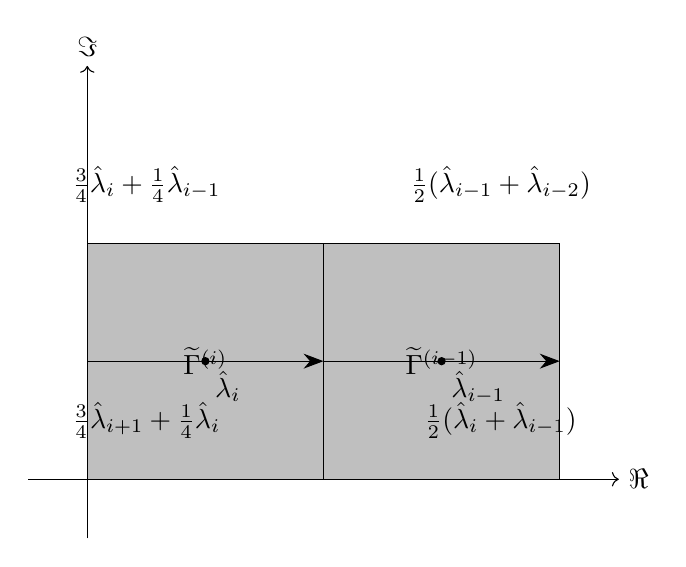
\begin{tikzpicture}[scale=1.5]
        % Axes
        \draw[->] (-0.5,0) -- (4.5,0) node[right] {$\Re$};
        \draw[->] (0,-0.5) -- (0,3.5) node[above] {$\Im$};
        
        % Curves
        \draw[fill=gray!50] (0,0) rectangle (2,2);
        \draw[fill=gray!50] (2,0) rectangle (4,2);
        
        % Labels for curves
        \node at (1,1) {$\widetilde{\Gamma}^{(i)}$};
        \node at (3,1) {$\widetilde{\Gamma}^{(i-1)}$};
        
        % Points
        \fill (1,1) circle (1pt) node[below right] {$\hat{\lambda}_i$};
        \fill (3,1) circle (1pt) node[below right] {$\hat{\lambda}_{i-1}$};
        
        % Arrows
        \draw[-{Stealth[scale=1.5]}] (0,1) -- (2,1);
        \draw[-{Stealth[scale=1.5]}] (2,1) -- (4,1);
        
        % Labels for points
        \node at (0.5,2.5) {$\frac{3}{4}\hat{\lambda}_i + \frac{1}{4}\hat{\lambda}_{i-1}$};
        \node at (3.5,2.5) {$\frac{1}{2}(\hat{\lambda}_{i-1} + \hat{\lambda}_{i-2})$};
        \node at (0.5,0.5) {$\frac{3}{4}\hat{\lambda}_{i+1} + \frac{1}{4}\hat{\lambda}_i$};
        \node at (3.5,0.5) {$\frac{1}{2}(\hat{\lambda}_i + \hat{\lambda}_{i-1})$};
        
        % Horizontal lines
        \draw (0,0) -- (4,0);
        \draw (0,2) -- (4,2);
        
        % Vertical lines
        \draw (0,0) -- (0,2);
        \draw (2,0) -- (2,2);
        \draw (4,0) -- (4,2);
    \end{tikzpicture}
    \caption{Choice of the curves $\widetilde{\Gamma}^{(i)}$ and $\widetilde{\Gamma}^{(i-1)}$ in the proof of Theorem \ref{Theorem2.3.1}.}
    \label{fig:curves}
\end{figure}

\end{document}